\newpage

\section{Wind Speed from Pitot Probe}

\subsection{Parts List}

\begin{enumerate}[itemsep=-5pt]
\item Laptop
\item CPX/CPB
\item USB Cable
\item Alligator Clips (x3)
\item Pitot Probe (Not included in kit at the moment so will need to buy this separately or borrow one)
\item Breadboard
\end{enumerate}

\subsection{Learning Objectives}
\begin{enumerate}[itemsep=-5pt]
\item Understand how pitot probes works
\item Understand the relationship between a voltage signal from a pitot probe to a pressure value
\item Understand the relationship between pressure and windspeed
\end{enumerate}

\subsection{Getting Started}

Although a CPX has numerous sensors built in, you can easily augment the capabilities of the CPX using either I2C or just the ADC on board the CPX. In this lab, if you purchased a \href{https://www.amazon.com/Hobbypower-Airspeed-MPXV7002DP-Differential-controller/dp/B00WSFWO36/ref=sr_1_3?dchild=1&keywords=Airspeed+sensor+kit&qid=1590532161&sr=8-3}{pitot probe} you will be able to do this assignment. Since you don’t need the pitot probe for very long you can always borrow one from some other team. Let’s talk about the hardware and the wiring to get this to work.
\begin{figure}[H]
  \begin{center}
    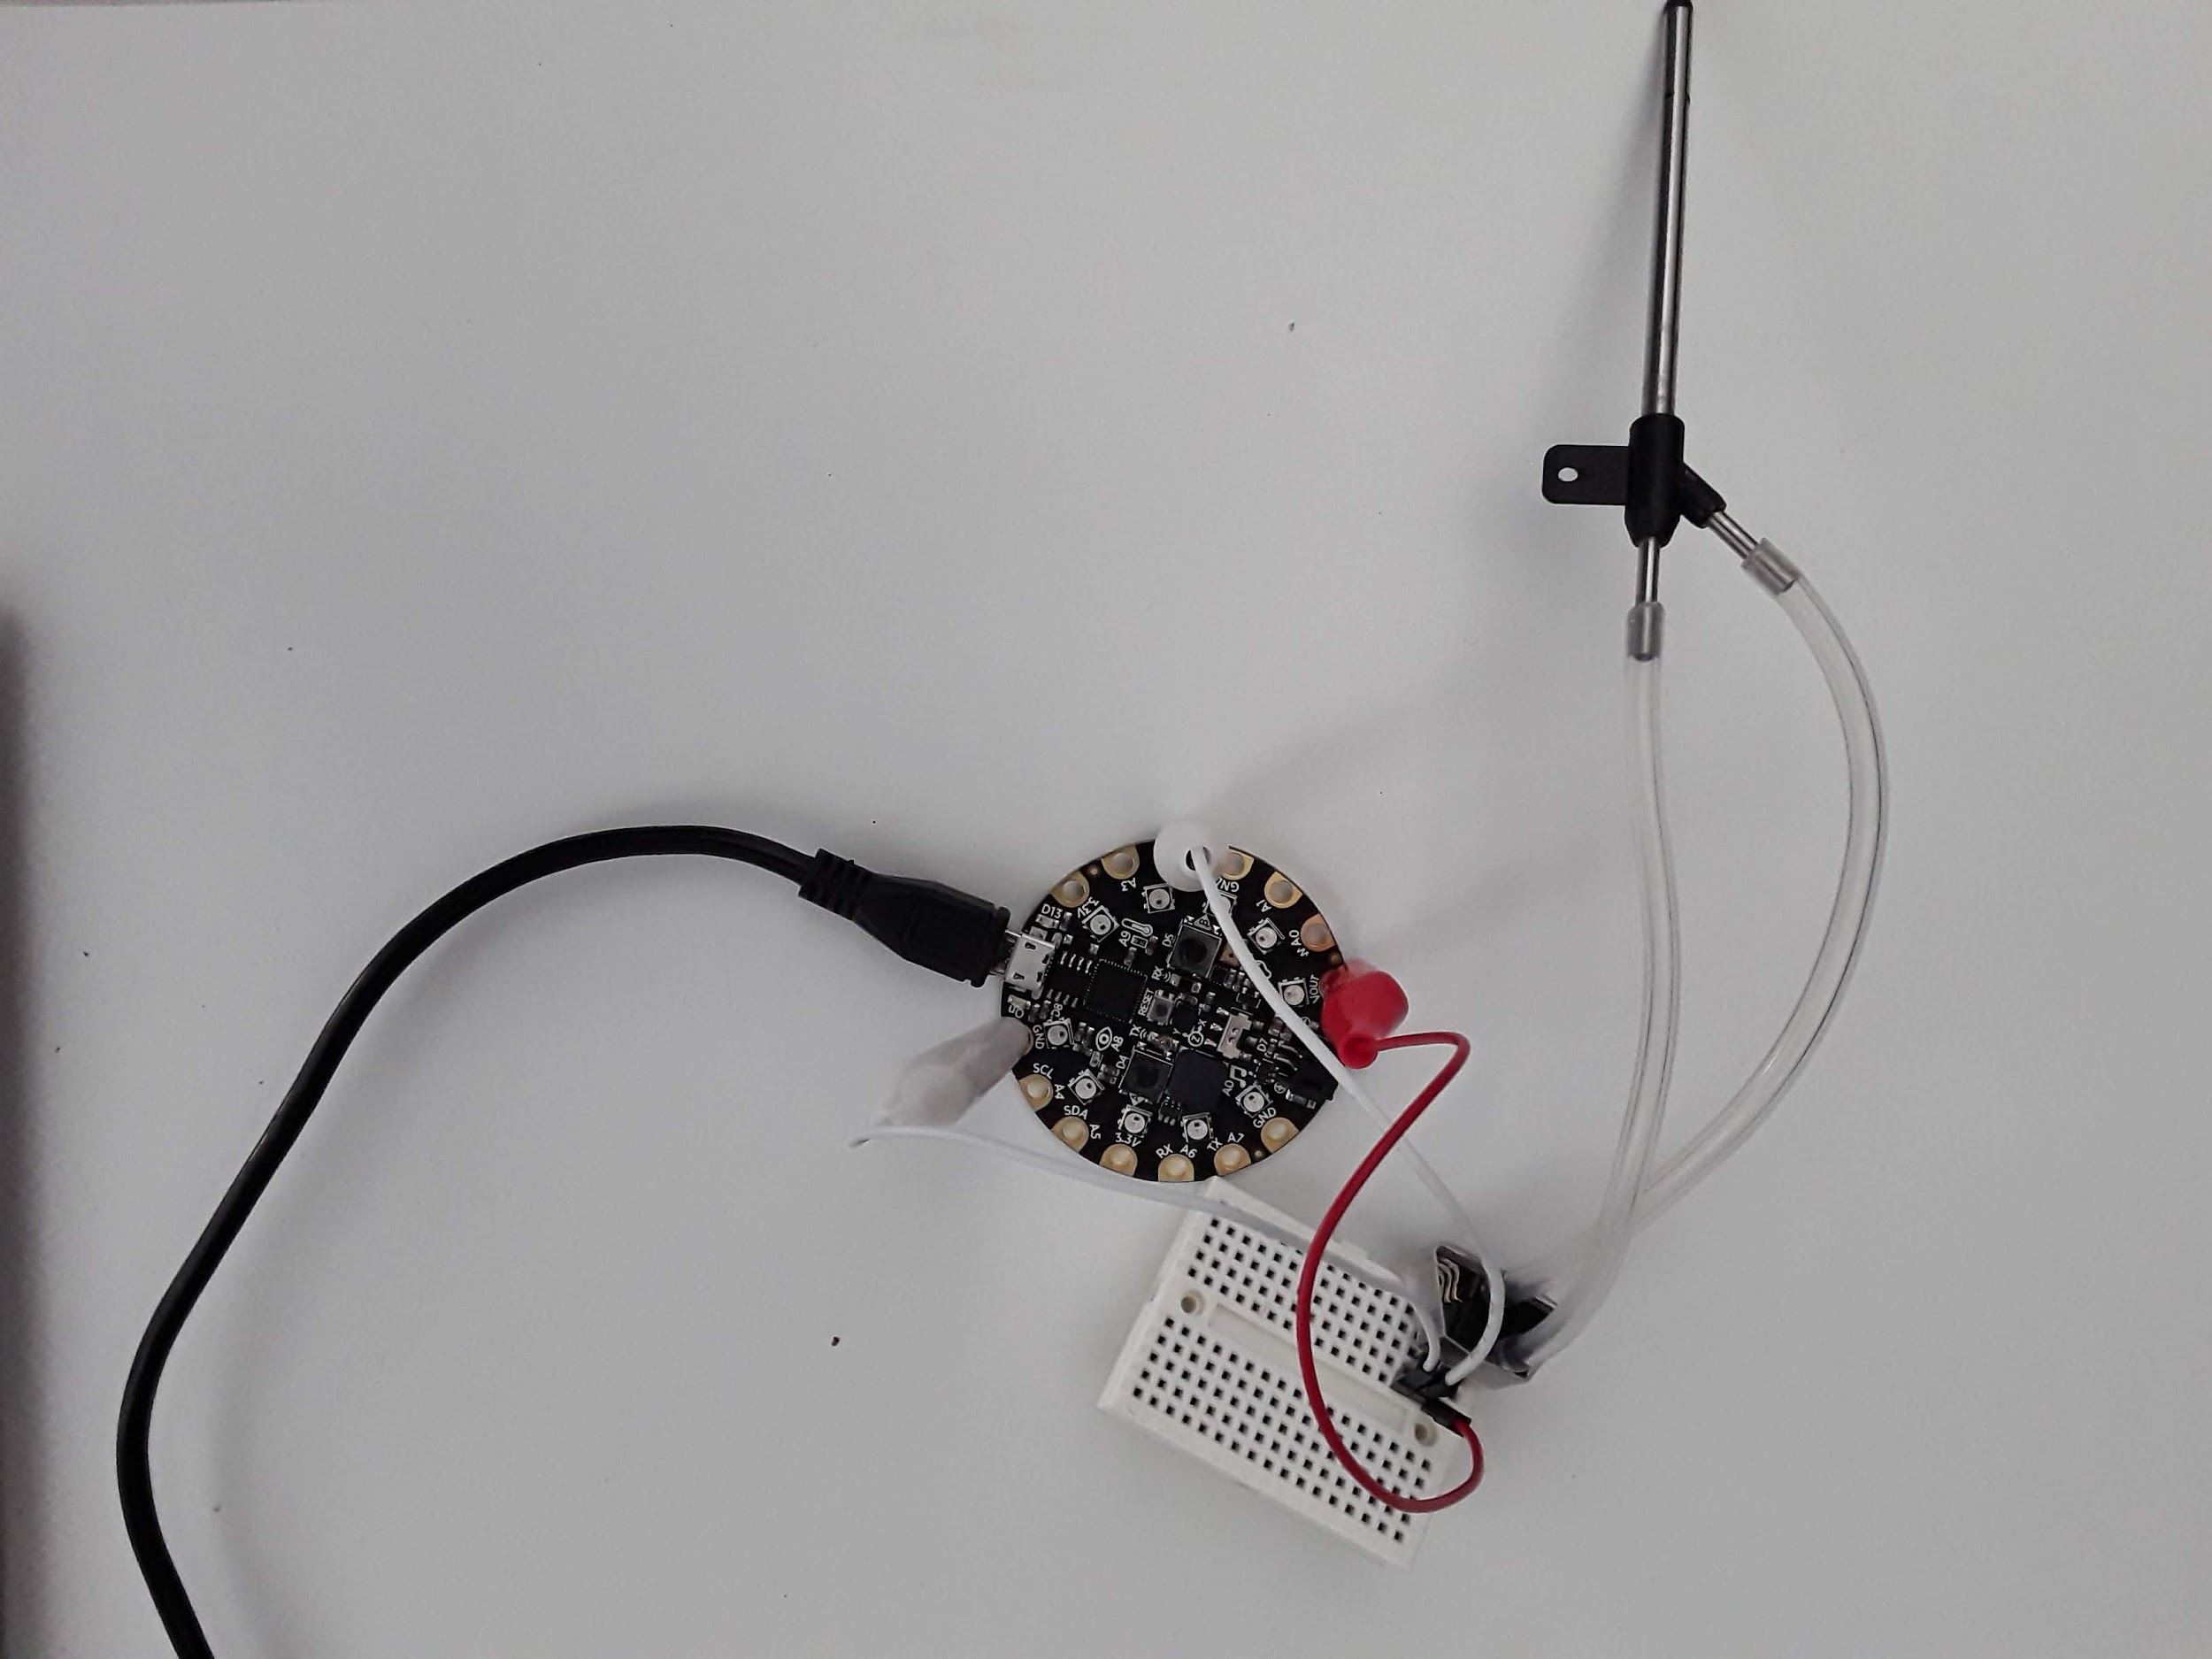
\includegraphics[width=\textwidth]{Figures/pitot_probe_circuit.jpeg}
  \end{center}
\end{figure}
The pitot probe has two pressure taps that measure ambient pressure and stagnation pressure. These taps move through two silicon tubes to a pressure transducer that has a strain gauge in separating both pressures. When the pressure on one side of the transducer is larger than the other, it will flex the membrane and create strain. This strain runs through a wheatstone bridge with a voltage offset to the pin labeled analog. The transducer has 3 pins, +5V, GND and Analog. It is pretty straightforward how to wire this up but remember that +5V needs to go to VOUT, GND to GND and Analog to any analog pin. I chose pin A2. At that point it’s very simple to just print the analog signal in bits to Serial. I’ve done this below. The code is the same \href{https://github.com/cmontalvo251/Microcontrollers/blob/master/Circuit_Playground/CircuitPython/Analog/analog_simple.py}{analog code} that we’ve used in the past.
\begin{figure}[H]
  \begin{center}
    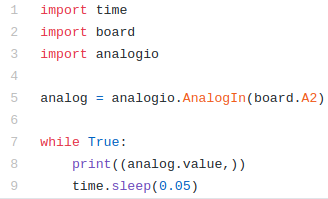
\includegraphics[width=0.5\textwidth]{Figures/analogio.png}
  \end{center}
\end{figure}
The goal of the experiment is to take pitot probe data for 15 seconds with no wind, then 15 seconds of data with a fan on and then 15 seconds of no wind data. You’ll need to use one of the datalogging methods (See chapter \ref{s:daq}) to log both time and pitot probe analog value. Once you have that data, import the data into Python on your desktop computer and convert the signal to windspeed. In order to convert the analog value to windspeed you need to first convert the analog value to voltage. Remember that the ADC on the CPX is going to convert the analog signal from the pitot probe to a digital output. So use this equation first to convert the analog signal (which I call D) to voltage. The 2 to the 16th power represents the 16 bit ADC.
\begin{equation}
V = \frac{3.3D}{2^{16}}
\end{equation}
Before converting Voltage to windspeed we need to first subtract off the bias from the pitot probe. I explain this process in this \href{https://www.youtube.com/watch?v=e4xs9Ky7_YI&feature=youtu.be}{accelerometer video}. I’ve done this project before and have posted a video on Youtube about \href{https://youtu.be/jSLIRC1cfvE}{Converting Pitot Probe Data to Windspeed}. {\bf \it There is a typo in the video. V1 is supposed to have a sqrt())}. Once you have computed the bias you can compute the change in pressure using the equation below which converts the change in voltage to Pascals ($V_b$ is the voltage bias you obtain when the wind is off). The data sheet states that the voltage is linearly proportional to pressure in Pascals which is nice.
\begin{equation}
P = 1000(V-V_b)
\end{equation}
Using pressure, the equation below can be used to compute windspeed, where U is the windspeed and the density at sea-level ($\rho$) is 1.225 $kg/m^3$.
\begin{equation}
U = \sqrt{\frac{2P}{\rho}}
\end{equation}
Using your data, create a plot of windspeed with time on the x-axis and windspeed on the y-axis. Some steps that might help you as you complete this project. First, have Mu plot the voltage coming from the pitot probe. If you’ve done everything right it will not be zero. The data sheet says there’s an offset voltage of 2.5V so you will hopefully get something around 50,000 when you don’t blow into the pitot probe. 50,000 multiplied by 3.3/$2^16$ is around 2.5V. Make a note of that average value you get so you can subtract it off later. Once you’ve verified you’re reading the pitot probe correctly, blow into the pitot probe and using the Plotter or Serial, verify that the analog signal increases. If the signal decreases, it means the pressure taps on the pressure transducer are backwards and you need to flip them. Either that or just flip the sign in your plotting routine on your computer but flipping the tubes might be easier for you. Hopefully when you do this lab you will get some data that looks like this. In this Figure you’ll see that when the fan wasn’t running the signal was something around 49,800 which is fine. It means your bias is around 2.5 volts. Every pitot probe and circuit will be different. You can then convert this signal to voltage then and then pressure and then finally wind speed.
\begin{figure}[H]
  \begin{center}
    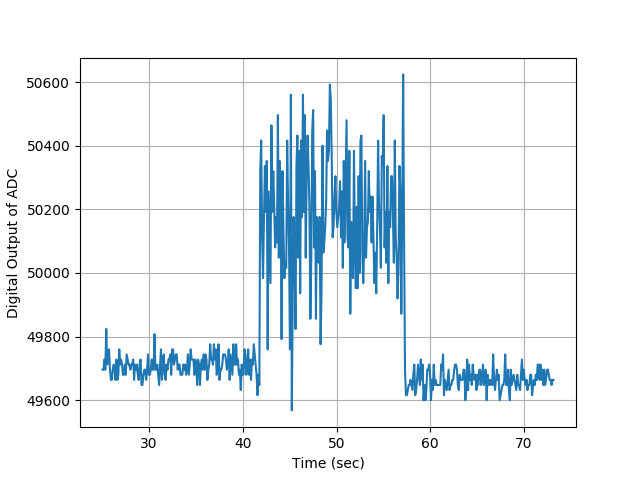
\includegraphics[width=\textwidth]{Figures/pitot_probe_data.png}
  \end{center}
\end{figure}
The code to accomplish this is relatively simple and a portion of the code is shown below. You’ll see that when I subtracted the bias from the voltage I also zeroed out any negative values. That is, any delta voltage less than zero was set to zero. A couple of things about this chart. The data from the pitot probe is super noisy which means attaching a \href{https://youtu.be/zTGa4sk6UZE}{complementary filter} is probably a good idea provided you don’t over filter the signal and run into \href{https://youtu.be/8F_8st_8MmA}{aliasing issues}. You can see that I implemented an offline complementary filter and plotted it in the orange line which helps the noise issue quite a bit. You’ll also notice that the noise is about 2 m/s. It turns out that pitot probes are actually not very accurate lower than about 2 m/s. They would be great for an airplane or you driving down the highway but they wouldn’t be very good to take wind data outside on a calm day.
\begin{figure}[H]
  \begin{center}
    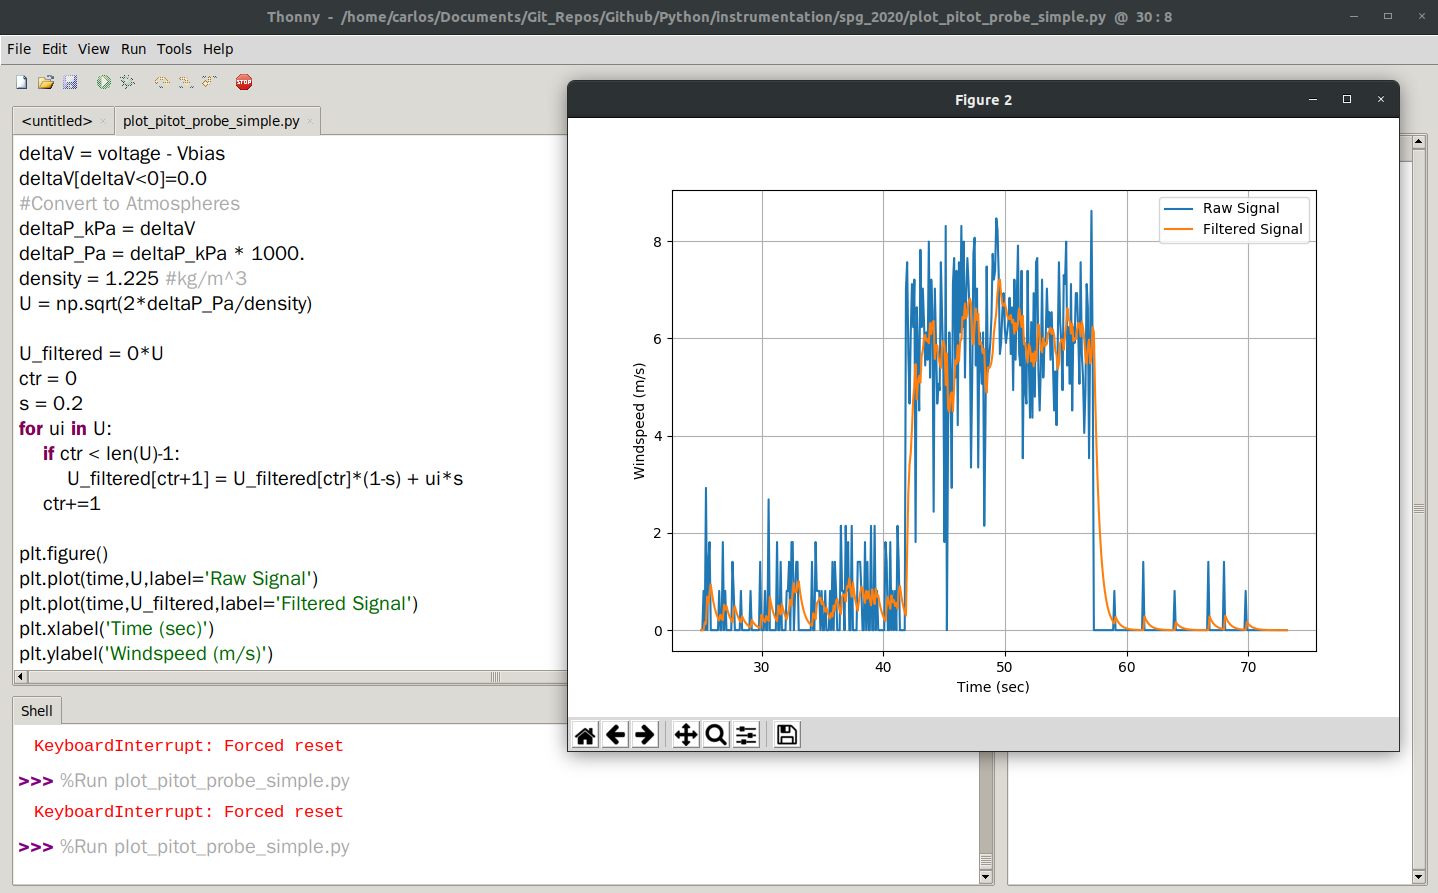
\includegraphics[width=\textwidth]{Figures/pitot_probe_final.png}
  \end{center}
\end{figure}

\subsection{Assignment}

Once you've done that upload a PDF with all of the photos and text below included. My recommendation is for you to create a Word document and insert all the photos and text into the document. Then export the Word document to a PDF. For videos I suggest uploading the videos to Google Drive, turn on link sharing and include a link in your PDF.

\begin{enumerate}[itemsep=-5pt]
\item If you borrowed a pitot probe return the pitot probe - Pass/Fail - If you don’t return the pitot probe you receive a zero
\item Include a video of you taking data and explaining the circuit (make sure you are in the video) - 50\%
\item Include a plot of the raw analog signal vs time just like I did above - 20\%
\item Include a plot of windspeed vs time as I did above - 20\%
\item Filter your signal using an offline complementary filter and include it in your plot like I did above - 10\%
\end{enumerate}